%------------------------------------------------------------------------------
% physor2016_template.tex - template to write a contribution for the PHYSOR 
% 2016 conference
% v2.0 20150508 Wilfred van Rooijen, University of Fukui
% v1.0 20130422 Wilfred van Rooijen, University of Fukui
%------------------------------------------------------------------------------
% Usage: this template file should be used ONLY with pdfLaTeX. Place this 
%        template file and the file physor2016.sty in the your working
%        directory. If you use bibtex, put physor2016.bst and physor2016.bib 
%        also in the working directory. If you have your own BiBTeX database
%        file, make a copy or link in your working directory and replace 
%        \bibliography{physor2014} with \bibliography{your_bib_file}.
%
% NOTE: when compiling your document, you may get warnings regarding
%       the versions of several of the style files used in the PHYSOR2016 tem-
%       plate. A warning is issued if the version on your computer is older than
%       the version requested in the style file. Under normal circumstances, 
%       there should be no problems but when in doubt, please check the log file
%       and update your LaTeX distribution if necessary. 
%------------------------------------------------------------------------------
\documentclass[12pt]{article}
%
% NOTE: use \documentclass[12pt,draft]{article} for your initial work. This 
%       will give you the "draft" mode:
%       - a black marker is printed for each "overfull hbox" (*)
%       - figures are not included (only the BoundingBox is indicated)
%       - hyperref is switched off
%
\usepackage{physor2016}
\usepackage{amsmath}
\usepackage{bm}
\usepackage{graphicx}
\usepackage{tikz}
\usepgflibrary{shapes.geometric}
\usepackage{booktabs}
\usepackage{siunitx}
\usepackage{epstopdf}
\usepackage{subcaption}
\usepackage{bigints}

\usepackage{tikz}

%  new definitions
\newcommand{\bs}[1]{\mathbf{#1}}
\renewcommand{\div}{\bs{\nabla}\! \cdot \!}
\newcommand{\grad}{\bs{\nabla}}
% extra space
\newcommand{\qq}{\quad\quad}
% common reference commands
\newcommand{\eqt}[1]{Eq.~(\ref{#1})}                     % equation
\newcommand{\fig}[1]{Fig.~\ref{#1}}                      % figure
\newcommand{\tbl}[1]{Table~\ref{#1}}                     % table
\newcommand{\sct}[1]{Section~\ref{#1}}                   % section
\newcommand{\app}[1]{Appendix~\ref{#1}}                   % appendix

\newcommand{\keff}{k_\textit{eff}}

\newcommand{\be}{\begin{equation}}
\newcommand{\ee}{\end{equation}}
\newcommand{\vn}{\vec{n}}
\newcommand{\vel}{\vec{\mathrm{v}}}
\newcommand{\adj}{\Phi^\dagger_0}
\newcommand{\tcr}[1]{\textcolor{red}{#1}}

%------------------------------------------------------------------------------

%------------------------------------------------------------------------------
% Define title. Use all CAPITALS.
%------------------------------------------------------------------------------
\title{IMPLEMENTATION OF THE IMPROVED QUASI-STATIC METHOD IN RATTLESNAKE/MOOSE FOR TIME-DEPENDENT RADIATION TRANSPORT MODELLING}
\author{ 
  \textbf{Zachary M. Prince$^\dagger$, Jean C. Ragusa$^\dagger$, Yaqi Wang$^\star$} \\
 $^\dagger$Department of Nuclear Engineering \\
  Texas A\&M University, College Station, TX, USA\\
  $^\star$Idaho National Laboratory\\
  \href{mailto:zachmprince@tamu.edu}{zachmprince@tamu.edu}, \href{jean.ragusa@tamu.edu}{jean.ragusa@tamu.edu}, \href{yaqi.wang@inl.gov}{yaqi.wang@inl.gov} 
}

%------------------------------------------------------------------------------
% The \shortauthor is printed on top of the even pages, and the \shorttitle
% is printed on top of the odd pages.
% Suggested format:
% - One author             : A. Author
% - Two authors            : A. Author \& B. Author
% - Three authors          : A. Author, B. Author \& C. Author
% - More than three authors: A. Author~et~al.
% If the title of your manuscript is very long, then make a short title such
% that it fits on one line in the header of the odd pages.
%------------------------------------------------------------------------------
\renewcommand{\shortauthor}      % Author's names here
           {Prince {\em et. al.}}  
\renewcommand{\shorttitle}       % Short title here
           {IQS in Rattlesnake}

%------------------------------------------------------------------------------
% Setup PDF info. This sets several values which are listed as the "properties"
% of the PDF file.
%------------------------------------------------------------------------------
\hypersetup{
  pdftitle=\shorttitle,
  pdfauthor=\shortauthor
}

%------------------------------------------------------------------------------
% Begin document
%
% \doublespacing -- This option will increase the line spacing, making it 
%                   easier to add written comments etc. Be sure to switch it 
%                   off when you make the final version!
%
% \linenumbers -- switches on line numbers, which are practical when reviewing 
%                 a manuscript. Switch off line numbers when you make your 
%                 final version. 
%------------------------------------------------------------------------------
\begin{document}

%\doublespacing
%\linenumbers

%------------------------------------------------------------------------------
% Make the titlepage and set the pagestyle to fancy throughout
%------------------------------------------------------------------------------
\maketitle

%------------------------------------------------------------------------------
%
%------------------------------------------------------------------------------
\section{Introduction}
\label{sect::intro}

The anticipated restart of Transient Reactor Testing (TREAT) Facility at Idaho National Laboratory (INL) has brought significant attention and opportunity to transient modeling.  TREAT, which was operational from 1954 to 1994, was designed to test nuclear fuels by subjecting them to various degrees of neutron pulses, from minor transients to accident cases.  Neutron transient modeling has always been computationally due to implicit time-stepping caused by the neutron velocity values. Even with the vast improvements in computing technology, straightforward discretization of neutron conservation equations remain computationally challenging for in real-world cases.  Therefore, methods that improve on computational speed significantly, at minimal detriment to accuracy, are highly desired. The Department of Energy (DOE) and INL have invested a substantial effort in modeling and simulation for TREAT.  This paper presents an implementation of the improved quasi-static (IQS) method for time-dependent neutron transport and diffusion equations with the multiphysics framework MOOSE \cite{moose}, notably its radiation transport application, RATTLESNAKE.

The improved quasi-static (IQS) method is a spatial kinetics method that involves factorizing the flux solution into space- and time-dependent components \cite{Ott_1969,Dulla2008}.  These components are the flux amplitude and its shape. Amplitude is only time-dependent, while the shape is both space- and time-dependent.  However, the impetus of the method is the assumption that the shape is only weakly dependent on time; therefore, the shape may not require an update  at the same frequency of the amplitude function, but only on macro-time steps. As opposed to other forms of quasi-static approximations, the IQS method is not an approximation; the shape is updated consistently.  The results of IQS may only differ from straightforward, temporal discretization because the time discretization truncation error in the shape increases with a larger time-step size. 

Implementing IQS to RATTLESNAKE in INL's MOOSE framework is an obvious endeavor to enable high-fidelity modeling of the TREAT facility. The rest of this summary will briefly describe the derivation of IQS (in the diffusion setting for brevity), its current application to RATTLESNAKE using the the MultiApp Picard iteration capabilities of MOOSE, and anticipated results to be generated by the full paper deadline.



%------------------------------------------------------------------------------
%
%------------------------------------------------------------------------------
\section{Background}
\label{sect::background}

In this Section, we recall the equations for the IQS method, starting from the standard multigroup diffusion equations written below:
\begin{align}
\frac{1}{v^g} \frac{\partial \phi^g }{\partial t} =& \frac{\chi_p^g}{\keff} \sum_{g'=1}^G (1-\beta) \nu^{g'} \Sigma_f^{g'} \phi^{g'} -  \left( -\div D^g \grad  + \Sigma_r^g \right) \phi^g  \nonumber \\
&  + \sum_{g'\neq g}^G\Sigma_s^{g'\to g} \phi^{g'}  + \sum_{i=1}^I\chi_{d,i}^g\lambda_i C_i \ , \quad 1 \le g \le G 
\end{align}
\be
\frac{dC_i}{dt} = \frac{\beta_i}{k_{eff}}\sum_{g=1}^G\nu^{g} \Sigma_f^g \phi^{g} - \lambda_i C_i \ , \quad 1 \le i \le I 
\ee
with
\be
\beta = \sum_{i=1}^I \beta_{i} 
\ee
Factorization is an important step in the derivation of the IQS method. The factorization approach leads to a decomposition of the multigroup flux into the product of a time-dependent amplitude ($p$) and a space-/time-dependent multigroup shape ($\varphi$):
\be
\phi^g(\vec{r},t)=p(t)\varphi^g(\vec{r},t)
\ee
To obtain the amplitude equations, the multigroup equations are multiplied by a weighting function, typically the initial adjoint flux ($\phi^*$), and then integrated over phase-space.  For brevity, the inner product over space will be represented with parenthetical notation:
\be
\int_D\phi^{*g}(\vec{r})f^g(\vec{r})d^3r=\left(\phi^{*g},f^g\right)
\ee
In order to impose uniqueness of the factorization, one requires the following:
\be
\sum_{g=1}^G\left(\phi^{*g},\frac{1}{v^g}\varphi^g\right) = \textit{constant}
\ee
After some manipulation, the standard point reactor kinetics equations (PRKE) for the amplitude solution are obtained:
%the amplitude and shape can be solved for by two systems of equations.  The amplitude can be obtained by solving 
\be
\frac{dp}{dt}=\left[\frac{\rho-\bar{\beta}}{\Lambda}\right]p+\sum_{i=1}^I\bar{\lambda}_i\xi_i
\ee
\be
\frac{d\xi_i}{dt}=\frac{\bar{\beta}_i}{\Lambda}-\bar{\lambda}_i\xi_i \quad 1 \le i \le I 
\ee
where the functional coefficients are calculated using the space-/time-dependent shape function as follows:
\be
\frac{\rho}{\Lambda}=
\frac{ \sum_{g=1}^G \left(\phi^{*g},\sum_{g'=1}^G\frac{\chi_p^g}{\keff} \nu^{g'} \Sigma_f^{g'}\varphi^{g'} + \sum_{g'\neq g}^G\Sigma_s^{g'\to g} \varphi^{g'} -\left( -\div D^g \grad  + \Sigma_r^g \right)\varphi^g\right)}
{\sum_{g=1}^G \left(\phi^{*g},\frac{1}{v^g}\varphi^g\right)}
\ee
%%
\be
\frac{\bar{\beta}}{\Lambda}=\sum_{i=1}^I\frac{\bar{\beta}_i}{\Lambda}=\frac{1}{\keff}
\frac{\sum_{i=1}^I\sum_{g=1}^G(\phi^{*g}, \beta_i\nu^{g} \Sigma_f^g \varphi^{g})}
{\sum_{g=1}^G \left(\phi^{*g},\frac{1}{v^g}\varphi^g\right)}
\ee
%%
\be
\bar{\lambda}_i=\frac{\sum_{g=1}^G(\phi^{*g},\chi_{d,i}^g\lambda_i C_i)}{\sum_{g=1}^G(\phi^{*g},\chi_{d,i}^gC_i)}
\ee

Finally, the shape equations are solved for the shape. The shape equations are similar to the orignal diffusion equations:
\begin{align}
\frac{1}{v^g} \frac{\partial \varphi^g }{\partial t} =& \frac{\chi_p^g}{\keff} \sum_{g'=1}^G (1-\beta) \nu^{g'} \Sigma_f^{g'} \varphi^{g'} -  \left( -\div D^g \grad  + \Sigma_r^g + \frac{1}{v^g}\frac{1}{p}\frac{dp}{dt}\right) \varphi^g  \nonumber \\
&  + \sum_{g'\neq g}^G\Sigma_s^{g'\to g} \varphi^{g'}  + \frac{1}{p}\sum_{i=1}^I\chi_{d,i}^g\lambda_i C_i \ , \quad 1 \le g \le G 
\label{eq:shape}
\end{align}
However, the amplitude and shape equations form a system of coupled equations: the coefficients appearing in the PRKEs depend upon the shape solution while the shape equation has a kernel dependent on amplitude and its derivative.  Because solving for the shape can be expensive, especially in two or three dimensions, it is attractive to make the assumption that the shape is weakly time-dependent so the shape can be computed after a multitude of PRKE calculations which is the root of IQS.  This is depicted schematically in \fig{fig:IQS}:
%
\begin{figure}[h]
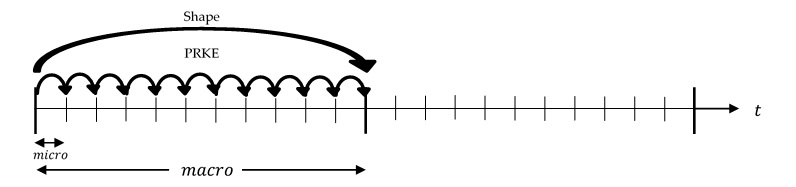
\includegraphics[width=\linewidth]{figures/IQS_visualization.jpg}
\caption{IQS method solution process}
\label{fig:IQS}
\end{figure}
%
Additionally, to improve consistency and accuracy, each macro time step can be iterated so the best shape is used to compute power at the micro time steps. Within the MOOSE framework,
nonlinear systems can be tackled in two manners: with Newton's method (usually, a preconditioned Jacobian-free version) and with Picard's iterations (fixed-point method). The latter is employed in the work. This iteration process must converge the shape such that the uniqueness condition $(\frac{d}{dt}\sum_{g=1}^G\left(\phi^{*g},\frac{1}{v^g}\varphi^g\right)=0)$ is preserved.


%------------------------------------------------------------------------------
%
%------------------------------------------------------------------------------
\section{Implementation in RATTLESNAKE}
\label{sect::implementation}

MOOSE, or Multiphysics Object-Oriented Simulation Environment, is a finite-element-based  framework developed by INL and is equipped with advanced nonlinear solvers.  Rattlesnake is a module of MOOSE meant for neutronics and radiation transport problems.  RATTLESNAKE is a radiation transport application within MOOSE and can be coupled to other physics via a Newton or a Picard approach. Implementing the IQS in RATTLESNAKE is meant to enhance its transient modeling capability.  RATTLESNAKE utilizes an action system which initiates kernels, user objects, and postprocessors; these typically need to be added manually to the input file, but due to the large phase-space of neutron transport approximations, an automated action system is invoked to add the required MOOSE objects. When implementing the IQS, the action system and its associated MOOSE objects need to be updated. For brevity, we describe the implementation in the case of the CFEM Diffusion action system; similar developments are carried out for the DFEM Diffusion action system, the $S_n$ Transport action system, \ldots We discuss the CFEM Diffusion action system in detail: 

\begin{figure}[h]
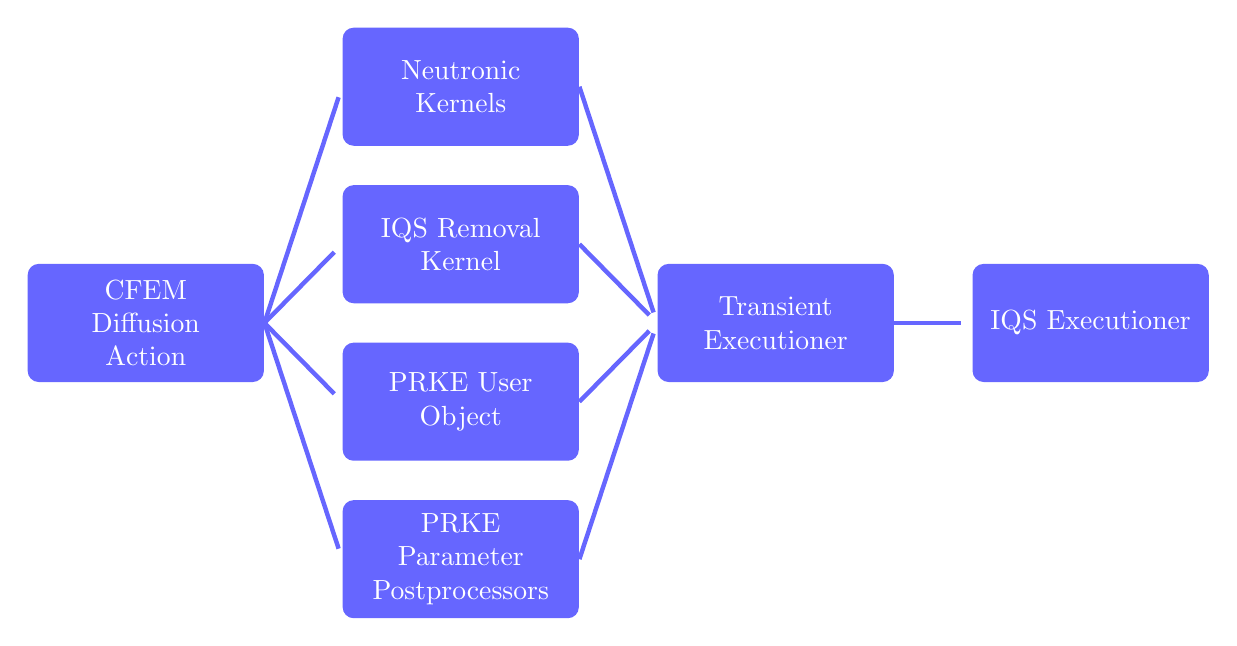
\begin{tikzpicture}[every node/.style = {shape          = rectangle, rounded corners, fill = blue!60, minimum width  = 3cm, minimum height = 1.5cm, align= center, text = white},blue edge/.style  = { -, ultra thick, blue!60, shorten >= 4pt}]
\node(0;0) at (0,0) {CFEM \\ Diffusion \\ Action};
  \node(1;3)  at (4, 3) {Neutronic \\ Kernels};   
  \node(1;1)  at (4, 1) {IQS Removal \\ Kernel}; 
  \node(1;-1)  at (4,-1) {PRKE User \\ Object}; 
  \node(1;-3) at (4,-3) {PRKE \\ Parameter \\ Postprocessors}; 
     \node(2;0)  at (8,0) {Transient \\ Executioner};
     	\node(3;0)  at (12,0) {IQS Executioner};
\foreach \j in {-3,-1,1,3}
  { \draw[blue edge] (0;0.east) -- (1;\j.west); }
\foreach \j in {-3,-1,1,3}
  { \draw[blue edge] (1;\j.east) -- (2;0.west);} 
\draw[blue edge] (2;0.east) -- (3;0.west);         
\end{tikzpicture}
\caption{CFEM Diffusion Action System Diagram}   
\label{Action}
\end{figure} 

%------------------------------------------------------------------------------
\subsection{Action System}

IQS derives its uniqueness from the executioner type; however, some additional changes needed to be carried out in the RATTLESNAKE/YAK action system in order to support IQS execution.   First, changes needed to be made in order to evaluate the shape equation.  The shape equation, after some manipulation, is very similar to the time-dependent flux equation, as seen in \eqt{eq:shape}.  To enable RATTLESNAKE to solve this shape equation in lieu of the standard diffusion equation, an additional removal kernel has to be instantiated to evaluate the quantity $\frac{1}{vp}\frac{dp}{dt}\varphi$ and added to FEM weak form  when the IQS executioner is selected.  Second, four postprocessors are created in order to calculate the PRKE parameters.  The parameter calculations were split into the following item: $\frac{\bar{\beta}_i}{\Lambda}$ numerator, $\bar{\lambda}_i$ numerator/denominator, $\frac{\rho}{\Lambda}/\frac{\bar{\beta}}{\Lambda}$ denominator, and $\frac{\rho-\bar{\beta}}{\Lambda}$ numerator.  The first three are relatively simple, only relying on material properties and solution quantities.  The $\frac{\rho-\bar{\beta}}{\Lambda}$ numerator requires the use of MOOSE's residual {\tt save\_in} feature, which saves the residual from a calculated kernel or boundary contribution in the shape evaluation to an auxiliary variable.  Finally, a user object was created to pull together all the postprocessor values and carryout the numerator/denominator divisions that were then passed to the executioner.

%------------------------------------------------------------------------------
\subsection{Executioner}

The IQS executioner derives from the Transient executioner in MOOSE.  The IQS executioner contains a loop over micro time steps that solves the PRKEs and then passes the values for $p$ and $dp/dt$ at times corresponding to the macro-time steps into the Transient executioner in order to solve for the shape equation at each macro step.  The PRKEs are solved with backward Euler within the Executioner for now but higher-order time integrators will be employed later.  The IQS executioner also supplements Transient?s Picard iteration process by adding its own error criteria for the IQS method: 
\be
\text{Error}_{\text{IQS}}=\left|\frac{\left(\phi^*_g,\frac{1}{v_g}\varphi_g^n\right)}{\left(\phi_g^*,\frac{1}{v_g}\varphi_g^0\right)}-1\right|
\ee
The use of the Picard iteration capability of MOOSE's executioner will enable solving the nonlinear IQS equations along with other nonlinearly coupled multiphysics (e.g., thermal-hydraulics) using different time step sizes for neutronics and the other coupled physics. 

%------------------------------------------------------------------------------
%
%------------------------------------------------------------------------------
\section{Preliminary results} 
\label{sect::results}

This section describes results of an example that tests the IQS implementation and shows its effectiveness on computation speed and accuracy.  We select a homogeneous one-group problem, subjected to a heterogenous material change (absorption cross-section change as a ramp in time for a subset of the geometry).


Figure~\ref{fig:power} shows the power at each macro time step, power is defined as the elemental integral of the flux.
\begin{figure}[!htbp]
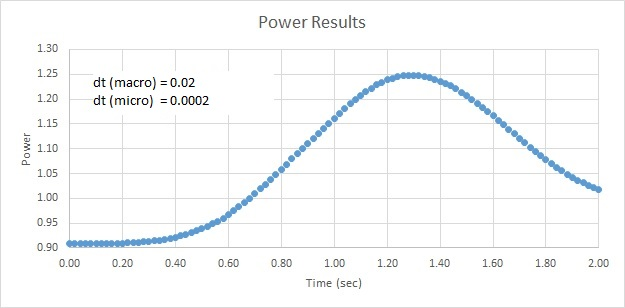
\includegraphics[width=\linewidth]{figures/power_results.jpg}
\caption{Power level computed as a Flux Integral Postprocessor value}
\label{fig:power}
\end{figure}


%------------------------------------------------------------------------------
%
%------------------------------------------------------------------------------
\section{Conclusions and Anticipated Additional Results} 
\label{sect::ccl}

We have implemented the IQS method within RATTLESNAKE, part of the MOOSE framework. The
implementation is complete for the CFEM Diffusion neutron equation and under testing for
DFEM Diffusion and $S_n$ transport equations. The application of IQS in MOOSE's Picard nonlinear solver was a relatively simple task using the object-oriented features of the framework. Once the implementation was completed for one action system, extension to other neutron discretizations was straightforward and elegant.  

For the final version of the paper, several multi-dimensional, multi-group transient test cases will be carried out using IQS (e.g., \cite{Yasinsky_1965,TWIGL_benchmark,LMW_benchmark}), including a multiphysics neutronics+heat conduction reactor dynamic problem \cite{ANL_BPB}. The
accuracy and time-to-solution will be compared with the IQS method and a straight temporal discretization of the original governing equations.


%------------------------------------------------------------------------------
%
%------------------------------------------------------------------------------
\bibliographystyle{physor2016}
\bibliography{references_IQS.bib}



\end{document}
